\documentclass[11pt]{scrartcl}
\usepackage[parfill]{parskip}
\usepackage{graphicx}
\usepackage{booktabs}
\usepackage{tabulary}
\usepackage{float}
\usepackage{eurosym}
\usepackage[T1]{fontenc}
\usepackage{selinput}
\usepackage[margin=2cm]{geometry}
\usepackage{enumitem,varwidth}
\usepackage[svgnames]{xcolor}
\usepackage{tikz}
\usetikzlibrary{shapes.geometric}
\usepackage{lmodern}

\parindent0em

\title{\textbf{Economic Aspects\\}}
\subtitle{Specific Report}
\author{Ricardo Garc\'ia Fern\'andez}
\date{\today}

\begin{document}

\maketitle

\tableofcontents

\newpage

\section{Title}

\par Me, my own company, or put another way: expertise in software development.

\par How to get experience developing FLOSS (Free Libre Open Source Software) and use it to get customers. What is a customer? for a single person is a client company itself, ie get a job at the company I want.

\par But we must bear in mind that you have to combine work experience and also have the 'extra' to be within a FLOSS development project. This is the extra quality that gives us this business model. Here we will focus on the development of a FLOSS tool by connecting with the community around us and use this as a gateway to the company.

\section{Target Description}

\par To begin we must draw a target, in this case we will make the goal of working in SpringSource\footnote{http://www.springsource.org/}, a division of VMware\footnote{http://www.vmware.com/} after being purchased in 2009.

\par \emph{SpringSource} is an application development framework for enterprise Java created in 2001 by Rod Johnson while he was writing a book or documented best practices with Java. In 2012 Rod Johnson left the company VMWare for joining the board of directors.

\par SpringSource is a \emph{FLOSS} (Free Libre Open Source Software) framework released under the Apache License Version 2.0\footnote{http://www.apache.org/licenses/LICENSE-2.0}. It has become an ecosystem modulated at the many options available for use in satellites framework and modules that can be used independently, this is the main strength of Spring, FLOSS and modularization be offered.

\par We need to be experts in Spring, that is our goal. Why Spring? we contribute some objective data.

\par In this summary concerning employment demand in IT sector found in \emph{Infojobs}\footnote{http://orientacion-laboral.infojobs.net/competencias-mas-demandadas-informatica-telecomunicaciones} we can draw in those figure~\ref{fig:req-profiles}:

\begin{figure}[H]
\begin{center}
  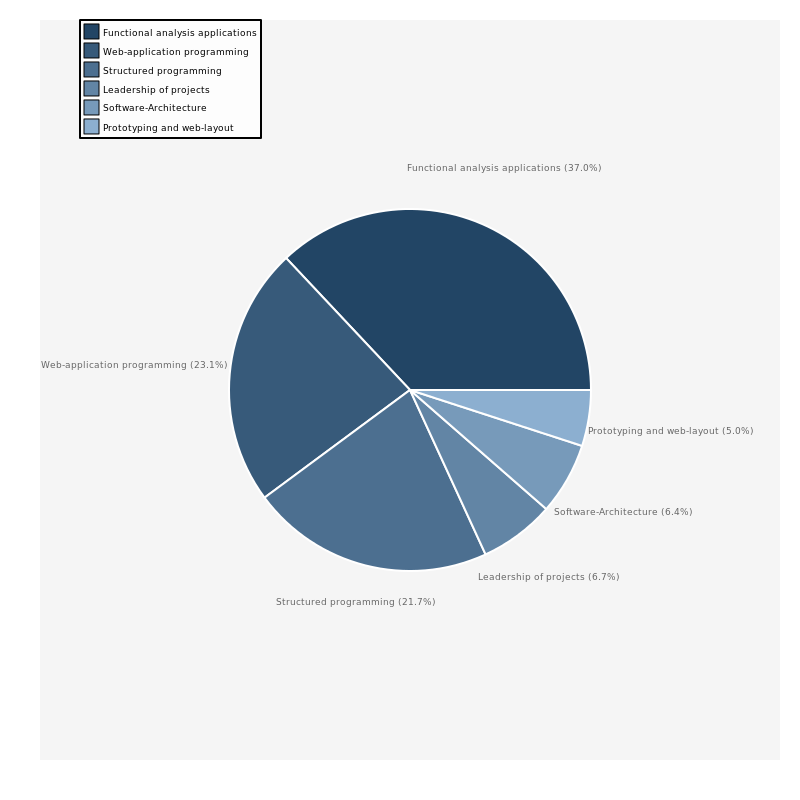
\includegraphics[width=0.7\textwidth]{images/requested-profiles-piechart.png}
  \caption{Software Development most popular profiles}
  \label{fig:req-profiles}
\end{center}
\end{figure}

\par And by the programming language Java can see hoards claims between Java and J2EE in figure~\ref{fig:req-languages}

\begin{figure}[H]
\begin{center}
  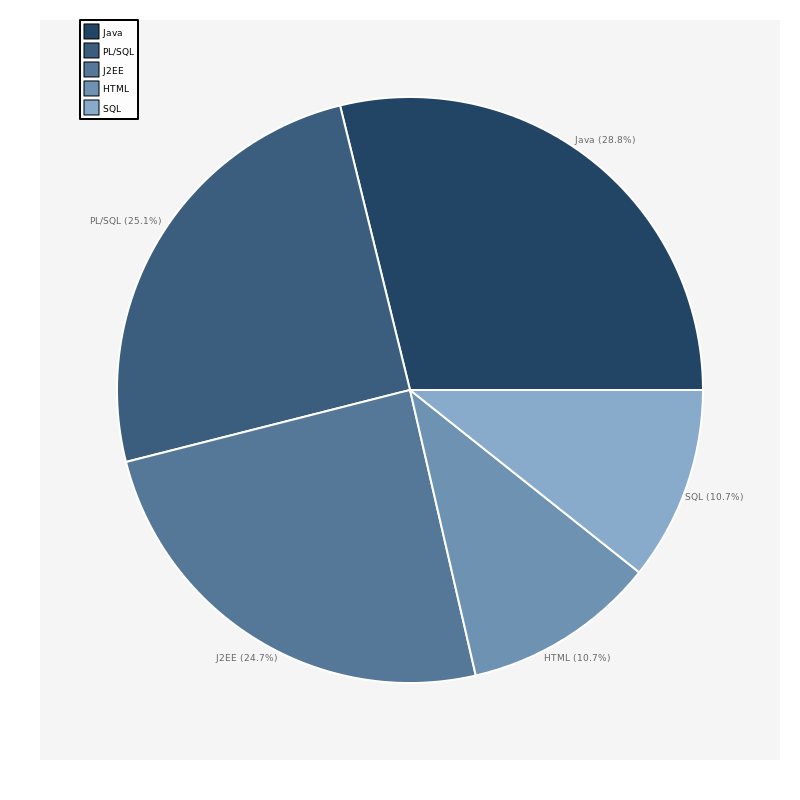
\includegraphics[width=0.7\textwidth]{images/requested-programming-language-piechart.png}
  \caption{Software Development most required languages}
  \label{fig:req-languages}
\end{center}
\end{figure}

\par Spring can be defined as a unification of both structured programming and Java web, therefore not only provides specific knowledge of the tool but it gives us knowledge about the most popular profiles on the software development world. And of course as you can see through this last graph, Java is a programming language freely and occupies a total of 60\% of demand.

\par This business model of \emph{expertise in software development} is based primarily on Technological Innovation, early adopters, and the classic; trial and error.

\par We can see how the community is divided in two main groups, on a fairly comprehensive guide tutoring in \emph{Get Started} section\footnote{http://www.springsource.org/get-started} and \emph{Get Involved}\footnote{http://www.springsource.org/get-involved}.

\subsection{Get Started}

This section of initiation can find all kinds of information on the Spring project learning divided into these six groups:

\begin{itemize}
    \item \emph{Start a Tutorial} - Beginners tutorials.
    \item \emph{Grab a Code Sample} - Examples functional.
    \item \emph{Ask a Question (Forums)} - Forum, active and important.
    \item \emph{Take a Class (Training)} - Spring University to learn to code.
    \item \emph{Read the Documentation} - Section important, not only for reading, but knowing how to use the documentation.
    \item \emph{Video Instruction} - Videos that show the tools and operation.
\end{itemize}

\par Try to cover different learning methods, readings, examples, videos, questions, online courses, which thus not only have a way of understanding and developers can choose the path that best suits them.

\par It can be defined as a learning community of Spring Framework within the same community Spring. A sub-community where users can learn and become teachers (using the nomenclature of teaching) around a forum that orbit other services communicating with each other.

\par This is our first step, get in touch with the user community the basic application. Because first you have to know that you are doing, what their possibilities and understand from the reasoning. You have to be in contact with the tool and use it. Use communication channels so we should immediately open an account at the forum and combine the first steps in the manual \emph{get started} with learning how to use the forum.

\subsection{Get Involved}

\par This is where the road begins regular or advanced user.

\par The presentation of this page shows an enthusiastic welcome comments from the community no matter the level of knowledge you have of Spring as this is a group dedicated to learning and sharing knowledge.

\par The structure is further defined by steps staggered with respect to user roles for this initial stage:

\begin{itemize}
    \item \emph{Join the conversation} - Encouraged to enter the ecosystem Spring for information everyday.
    \item \emph{Help other users (And get help when you need it too)} - Use the forums to help or receive help from others and also using social network Stackoverflow\footnote{http://stackoverflow.com/} con los tags \emph{spring} y \emph{spring-mvc}.
    \item \emph{Report issues} - Invites report bugs or improvements through Spring issue tracker JIRA\footnote{http://jira.springsource.org/}.
    \item \emph{Track the latest features and test them out} - Active use of JIRA to test new features or errors helping the community to solve.
    \item \emph{Contribute code} - We housed the Spring code repository on GitHub\footnote{http://github.com/SpringSource} to use the latest version of the source code published for through tickets and Github defined in relation to the JIRA can provide a solution or improvement through your source code and if it solves or meets the requirements, you will be part of the group of users who contribute code to Spring Framework by signing a contract of contributor\footnote{https://support.springsource.com/spring\_committer\_signup} to the project.
    \item \emph{Attend (or give) a talk at a local user group} - Encourages the developer to attend talks on Spring or to be the speaker of the same talk to your nearby groups of developers, noting that Spring appreciates this task, help promote the proper use of its Framework directly offering his help.
    \item \emph{Attend a spring-related conference} - As a last point gives us information about the annual conference of Spring which reports and discusses the improvements and / or developments of Spring joining it to be more in touch with the community.
\end{itemize}

\par This section is where we can really see the potential of FLOSS projects regarding proprietary. The community that exists around the project and the importance it gives.

\par The most important points of collaboration in this guide are those that have to help us to achieve our goal. We highlight the facilities offered to interact with them, which private companies can only find their successful cases with their private technology, the name of an application that have been developed and some pictures taken from an image bank with smiling people working with no nothing to do with business. Where it appears that the stereotype is the predominant guide.

\par However in FLOSS companies like Spring, are more real/human, real people who work there as you can get in touch with them through different communication channels that provide and more importantly, they also know the importance these channels. And if there are pictures on the website, at least they themselves or so says wikipedia.

\section{What is our roadmap?}

\par After gathering information about Spring technology, what we have to do now?

\par We have to know what kind of workers the company seeks, to retrieve this list published on their website\footnote{http://jobs.vmware.com/search?q=springsource}. To focus our specialization according to the descriptions given in the job, we are left with something specific, we need to know who ask and how they ask.

\par \emph{Wield it for our personal use and learn to use it like an expert.}

\par Today internet (although it sounds cliche but it's true and you have to highlight it) has become a window to information and communication (from the beginning are the two premises from which it was created, so the reference to cliche) so we have to use it to give visibility and generate an upstroke (or not) in the acquisition of knowledge to be shared. For this we need to use tools that are available to anyone with a computer and internet connection:

\begin{itemize}
    \item \emph{email}: you have to start with the basics and do not take anything for granted, we need an email. The email is the cornerstone of this system, all the other tools you can say that are somewhat heirs of this technology.
    \item \emph{Blog}: Open a blog or post to a blog is existing own a very good idea because it gives us a record of our main interests. In the blog can post concept tests as guides to be used by people, it is always easier to replicate something functional. As we publish the entries, social networks play an important asset. So you have to be inside them and professionalize your profile according to the requirements of Spring.
    \item \emph{Social Networks}: Twitter\footnote{http://twitter.com/\#!/springsource} as official channel in Spring. Post each tutorial linked to official Spring user and all its members. This is a way to leave a trail technological and get user feedback.
    \item \emph{github}\footnote{https://github.com}: GitHub Helps people build software together. A Repository of Repositories, composed developer community which publishes public repositories helping the dissemination of content to increase the interaction between developers. This site is to help us to publish the proof of concept we make of the tool. The uses and applications that create the same and more importantly, to interact with other developers contributing to their projects.
    \item \emph{StackOverflow}\footnote{http://stackoverflow.com}: A bill to interact with users on this social network Spring above. This network is important because it will bring together many (if not all) development technologies, making it a good place to gain and share knowledge and gain some respect in the community so that it can become a good cover letter.
    \item \emph{Spring account}: an account for the forum and the issue tracker. This is the most important consideration because it is giving us access to the network of Spring. Forum and foremost JIRA. We have to become familiar with JIRA, here begins our race to become experts. For starters, if you find an error, report it. Then when we have become familiar with the tool (Spring, any of its modules) can start to take care on our own to fix bugs found by users and attach them to the issue. Thus, if we are consistent and efficient, we will be in Spring committer permits, a big step for the business strategy.
\end{itemize}

\par All this information must be unified in an orderly manner in order to be useful, we will see a little guide to how to get the most out of presenting itself as an active and interested in Spring.

\par The deadline of the business plan is set in a year. A year spent learning technology and gain online visibility.

\par From here, we must unify our annual tour. Whether we have become committers Spring or not. The next step is to prepare social curriculum, took a year working on this project. Starting submit an application for a job in Spring, not to mention the contacts we have made during the year. Ask the developers of the project if people are looking for and where would you send your resume.

\par Portraying the year dedicated to being committer Spring makes learn, as does a community, being in a FLOSS project, group work, new technologies, reason why. So all this learning experience is a positive turn. If not go into VMWare, we won learning how to work Spring, this also applies to us and move on to other satellite companies in the universe Spring.

\section{Not a new model}

\par This is not a new business model. It is based on open innovation and knowledge ecosystem and opportunities arising around.

\par Here's a few examples of companies that have specialized in developing technology FLOSS and some users that follow that path to be hired by a company using FLOSS public knowledge:

\begin{itemize}
    \item Iglalia\footnote{http://www.igalia.com/}: is an open source consultancy specialized in the development of innovative projects and solutions. The contribution of the company in various FLOSS projects such as Webkit, is established for one of the leading companies that provides this tool. Of course that is behind Google and Apple. As seen in RoR \emph{Ohloh.net} recent contributions in Webkit repository\footnote {http://www.ohloh.net/p/WebKit/contributors?query=igalia\&sort=commits}.
    \item \emph{OpenStack Effect}: OpenStack\footnote{http://www.openstack.org/} is a FLOSS project for building private and public clouds. This project has grown at an exponential rate in two years since its publication by Rackspace and NASA. It serves as a mirror to extract the method of how to become an expert in technology (as an individual) and be hired by a company. In this race the developers, in this case we will customize, compete to specialize in this technology. The amount of resources (provided by companies in this case) that is bringing together OpenStack is very large so if you excel as a developer, which is not an easy task, companies may opt for this technology, try to hire you.
    \item \emph{FOSDEM} is a free event that offers open source communities a place to meet, share ideas and collaborate. This year (2nd February 2013) is a talk related to this business model; '\emph{Get a Python job, work on OpenStack}'\footnote{https://fosdem.org/2013/schedule/event/openstack/}. Very interesting and I'll write about it.
\end{itemize}

\par These examples illustrate the journey that we have to keep learning a technology FLOSS to become an expert ergo get a job at a company that interests you, thus, get the client you are looking for.

\section{Advantages and Drawbacks}

\par Like any business plan, we need to disseminate to look beyond a specific plan, so we summarize the advantages and drawbacks of this model

\subsection{Advantages}

\begin{itemize}
    \item We will learn to work in community. Work group.
    \item We became experts.
    \item Access cutting-edge technology.
    \item Learning a new programming language. Or upgrade to a learning community share.
    \item Learn to handle tools for other purposes.
    \item Being in touch with more professionals, developers. Meet other viewpoints.
    \item Choosing the type of client we want to obtain.
    \item Avoid the means of production, able to survive on your own.
\end{itemize}

\subsection{Drawbacks}

\begin{itemize}
    \item We focus on technology. We focus on a single technology, depend on it.
    \item Community strict and difficult to access as a committer.
    \item Availability time, yours and ours. 
    \item Lower the use of technology. The technology gradually lose their status due to external causes.
    \item Lack of documentation. Documentation unclear and scattered
    \item Lack of examples. No 'Hello world'.
    \item Unifying distributed information channels, blog, repository, etc, on a resume (cv). We must concentrate on this part but also requires investing time
\end{itemize}

\subsection{SWOT Matrix}

\par Having located the advantages and drawbacks, this information can be translated through a SWOT Matrix\footnote{http://www.swotmatrix.com/} - \emph{(Strengths, Weaknesses, Opportunities, Threats)} - to be more easily readable and interpretable.

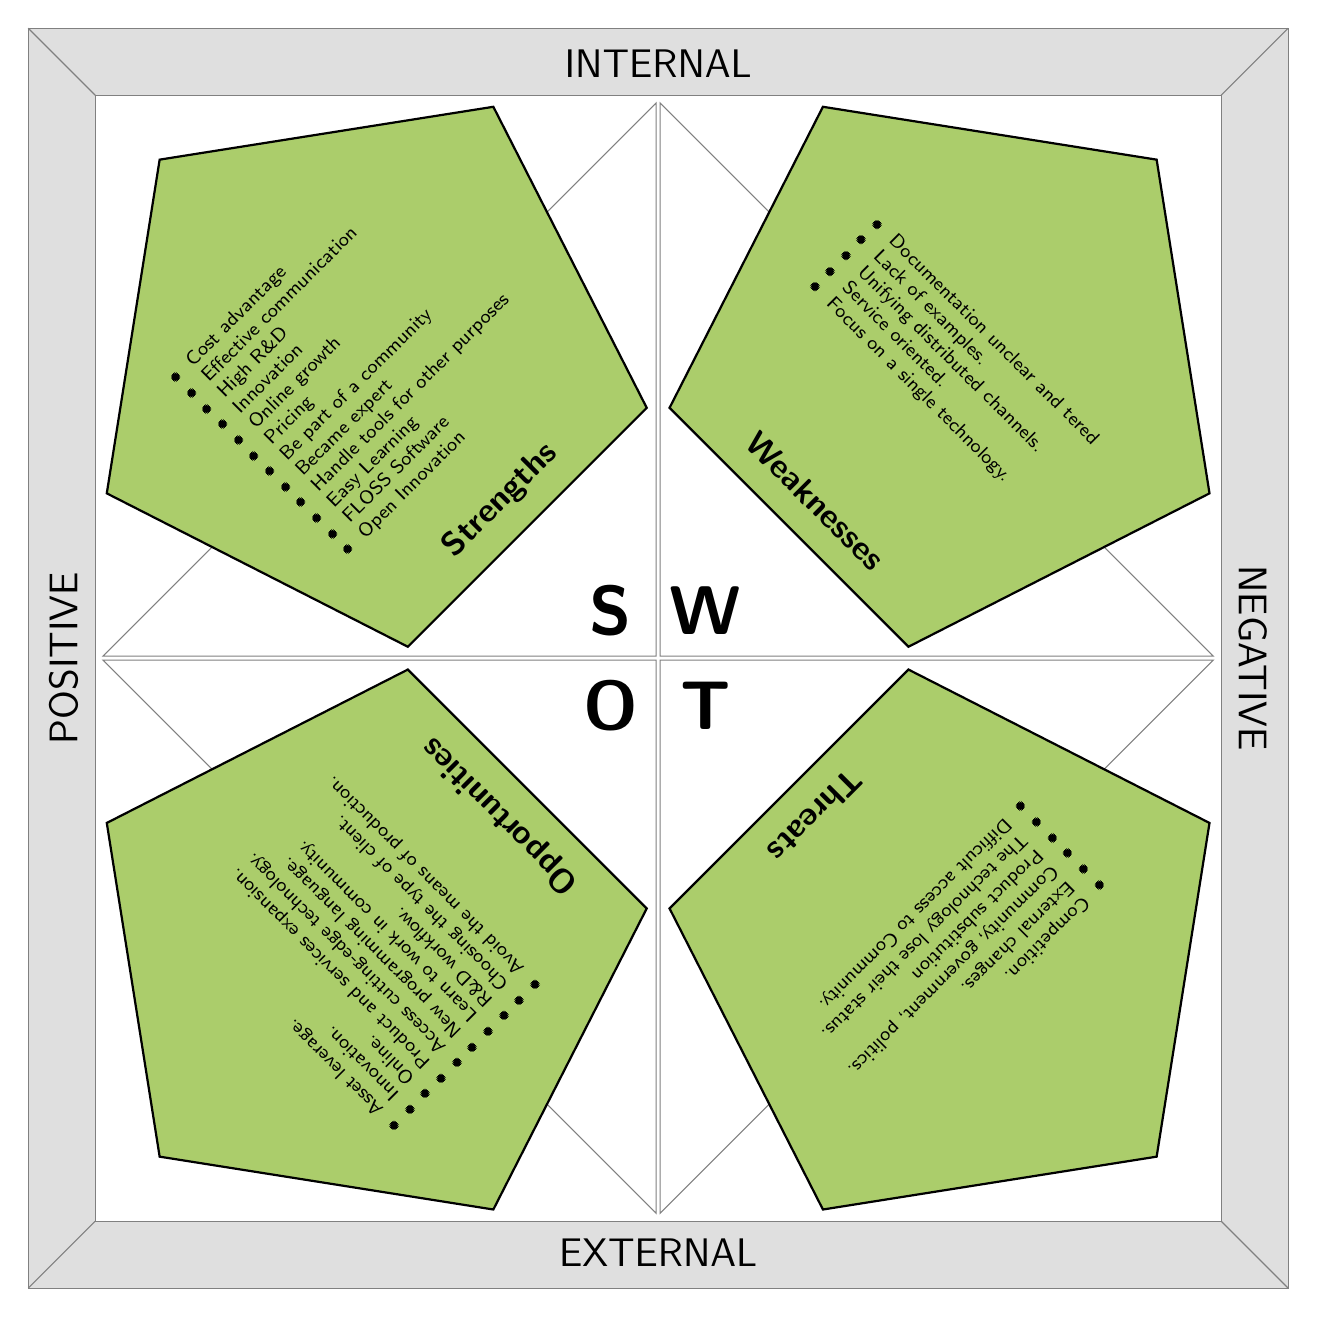
\begin{tikzpicture}[
    pentagon/.style={%
      shape=regular polygon,
      regular polygon sides=5,
      minimum size=7.3cm,
      inner sep=-1mm,
      draw,
      fill=DarkSeaGreen!75!yellow
    },
    font=\scriptsize\sffamily,
    thick
]
\filldraw[thin,gray,fill=gray!25] (-8,-8) rectangle (8,8);
\filldraw[thin,gray,fill=white] (-7.15,-7.15) rectangle (7.15,7.15);
\draw[thin,gray] (7.15,7.15)--(8,8) (-7.15,7.15)--(-8,8) (-7.15,-7.15)--(-8,-8) (7.15,-7.15)--(8,-8);

% Strengths
\draw[thin,gray] (-0.025,0.025)--(-7.05,0.025)--(-0.025,7.05)--cycle;
\node[pentagon,rotate=45] at (-3.75,3.75) {
    \begin{varwidth}{\linewidth}
        \begin{itemize}[leftmargin=*,noitemsep]
            \item Cost advantage
            \item Effective communication
            \item High R\&D
            \item Innovation
            \item Online growth
            \item Pricing
            \item Be part of a community
            \item Became expert
            \item Handle tools for other purposes
            \item Easy Learning
            \item FLOSS Software
            \item Open Innovation
        \end{itemize}
    \end{varwidth}
};
\draw (-2,2) node[rotate=45] {\large\textbf{Strengths}};

% Weaknesses
\draw[thin,gray] (0.025,0.025)--(7.05,0.025)--(0.025,7.05)--cycle;
\node[pentagon,rotate=-45] at (3.75,3.75) {
    \begin{varwidth}{\linewidth}
        \begin{itemize}[leftmargin=*,noitemsep]
            \item Documentation unclear and tered
            \item Lack of examples.
            \item Unifying distributed channels.
            \item Service oriented.
            \item Focus on a single technology.
        \end{itemize}
    \end{varwidth}
};
\draw (2,2) node[rotate=-45] {\large\textbf{Weaknesses}};

% Opportunities
\draw[thin,gray] (-0.025,-0.025)--(-7.05,-0.025)--(-0.025,-7.05)--cycle;
\node[pentagon,rotate=135] at (-3.75,-3.75) {
    \begin{varwidth}{\linewidth}
        \begin{itemize}[leftmargin=*,noitemsep]
            \item Asset leverage.
            \item Innovation.
            \item Online.
            \item Product and services expansion.
            \item Access cutting-edge technology.
            \item New programming language.
            \item Learn to work in community.
            \item R\&D workflow.
            \item Choosing the type of client.
            \item Avoid the means of production.
        \end{itemize}
    \end{varwidth}
};
\draw (-2,-2) node[rotate=135] {\large\textbf{Opportunities}};

% Threats
\draw[thin,gray] (0.025,-0.025)--(7.05,-0.025)--(0.025,-7.05)--cycle;
\node[pentagon,rotate=-135] at (3.75,-3.75) {
    \begin{varwidth}{\linewidth}
        \begin{itemize}[leftmargin=*,noitemsep]
            \item Competition.
            \item External changes.
            \item Community, government, politics.
            \item Product substitution
            \item The technology lose their status.
            \item Difficult access to Community.
        \end{itemize}
    \end{varwidth}
};
\draw (2,-2) node[rotate=-135] {\large\textbf{Threats}};

\draw(0,-7.55) node {\Large EXTERNAL};
\draw(0,7.55) node {\Large INTERNAL};
\draw(-7.55,0) node[rotate=90] {\Large POSITIVE};
\draw(7.55,0) node[rotate=270] {\Large NEGATIVE};
\draw(-0.6,0.6) node {\Huge\textbf{S}}; 
\draw(0.6,0.6) node {\Huge\textbf{W}};
\draw(-0.6,-0.6) node {\Huge\textbf{O}};
\draw(0.6,-0.6) node {\Huge\textbf{T}};
\end{tikzpicture}

\section{Useless without FLOSS}

\par FLOSS envelops everything, communication, innovation, knowledge sharing and dissemination of knowledge above.

\par FLOSS allows us to learn, as in this case the working methodology of SpringSource. Being a FLOSS community teaches its methodology and its strengths.

\par But if they were not a FLOSS project, this plan would radically change starting with the cost of training. We can build on the price of courses that lead to the examination of It costs us, 2590\euro each course, there are four:

\begin{itemize}
    \item Spring Core (CORE)
    \item Spring Web (SWEB)
    \item Enterprise Integration with Spring (EIS)
    \item Hibernate with Spring (HS)
\end{itemize}

\par A total of 10360\euro initial investment to get a Spring certification. That is totally valid, of course. We just started and there is a difference of 10360\euro, plus we adhere to their particular program, that does not mean it's bad, but there are possibilities of getting a job there too. Thanks to FLOSS projects, we can work with latest technology innovations.

\par Through the Open Knowledge and the use we have to give to the community, the learning curve is better because we can get better information through the community. Moreover, we must learn to distinguish good information from bad, learn to ask, learn to interact, to learn after all. This tour is based on learning and knowledge sharing. A small example would be, ask a teacher a question and course overnight wait for answer, or ask a question in the Spring forum and to receive a valid response instantly due to the globalization of the Internet and it does not depend schedules.

\par This model is heavily based on meritocracy. \emph{Meritocratic}: of meritocracy, based on personal merit\footnote {http://www.wordreference.com/es/translation.asp?tranword=meritocratic}. It requires a commitment and a way of working that gradually expands. Meritocracy rewards knowledge among specialists of the same, is not new, it's like a prize chosen by writers for writers, so people skilled in the art, from anywhere in the world, appreciates your merits, which in the end out is essential in science.

\begin{thebibliography}{9}

\bibitem{spring-community}
  Spring community analysis,\\
  Ricardo Garc\'ia Fern\'andez,\\
  http://www.youtube.com/watch?v=K\_nnmQE9jUA

\bibitem{}
    Developing 'Free/Libre/Open Source Software (FLOSS)' - A Market Driven Investment - November 10, 2008,\\
    Nicolas Jullien,\\
    Telecom Bretagne; M@rsouin (M\^ole Amoricain de Recherche sur la Soci\'et\'e de l'information et les Usages d'Internet),\\
    http://papers.ssrn.com/sol3/papers.cfm?abstract\_id=1298954

\end{thebibliography}

\end{document}